%!TEX program = xelatex
%!BIB program = bibtex
\documentclass[cn,black,12pt,normal]{elegantnote}
\usepackage{float}
\usepackage{hyperref}
\usepackage{amsmath}
\usepackage{amsfonts}
\usepackage{amssymb}
\usepackage{siunitx}[=v2]
\usepackage{fancyhdr}
\usepackage{newtxtext}
\usepackage{algorithm}
\usepackage{algorithmic}
\newcommand{\uct}[1]{\textsuperscript{\textsuperscript{\cite{#1}}}}
\renewcommand{\tablename}{\textbf{Table}}
\renewcommand{\figurename}{Figure.}
\renewcommand{\refname}{References}
\renewcommand{\contentsname}{Contents}
\renewcommand{\versiontext}{Version: }
\renewcommand{\updatetext}{Update: }
\PassOptionsToPackage{no-math}{fontspec}
\lstset{basicstyle=\footnotesize\ttfamily\color[RGB]{50,0,130},numbers=none,frame=trBL}

\sisetup{mode=text}
\sisetup{range-phrase = \text{ \textasciitilde }}
\pagestyle{fancy}
\fancyhead[L]{School of Software Engineering, Tongji University}
\fancyhead[R]{Data Structure Projects}
\renewcommand{\headrulewidth}{1pt}

\title{Evaluation of expressions\\表达式计算}
\author{1951510\; 姜文渊}
\institute{\small \url{https://github.com/jwyjohn/Jwy_DataStructureHomework}}
\version{0.50}
\date{\today}

\begin{document}

\maketitle

\textbf{Data structure involved:} Tree, Stack, String

\tableofcontents

\newpage

\section{Introduction}

One of the main purposes of computers is to evaluate arithmetic expressions much faster than human beings. One of the problems people met when trying to design and use computers to do arithmetic calculation is that, the expressions we human write is not friendly to the computers. Thus, to make computers understand what a user want to do, a conversion of languages has to be done.

One of the machine-friendly expression languages is known as the Reverse Polish notation (RPN or postfix expressions).\uct{wiki:Reverse_Polish_notation} Like the ordinary expressions we wrote, postfix expressions have operaters and oprands, but in an order that is unfamiliar to common people, in which operators follow their operands, in contrast to Polish notation (PN), in which operators precede their operands. It does not need any parentheses as long as each operator has a fixed number of operands. For example, the expression \lstinline{2 + 3 * 4} would be \lstinline{2 3 4 * +} as postfix expressions.

The process of converting expressions was previously done by programmers, but due to the progress on formal language and automaton theory, we now have methods to write programs to do the conversion. More specificly, a model called Abstract Sytax Tree (AST) is generated from a user's input, and other forms of expressions is generated from the Abstract Sytax Tree. Evaluation of an expression can be done using postfix expressions or done by recursively processing the AST.

In this demo, the author built a demo to process a type of simple but common expressions with integers, "$+$", "$-$", "$\times$", "$\div$", "$($" and "$)$". A AST will be generated, while the value, the postfix expression, infix expression will be outputed, if the expression is vaild.

A vaild expression should follow the grammar below:

\begin{lstlisting}
exp     :	term			    
		|   exp '+' term		
		|   exp '-' term		
		;
 
term	:	digit               
		|   term '*' digit		
		|	term '/' digit		
		;
 
digit	:	NUM                 			
		|   '(' exp ')'        
\end{lstlisting}

For example, the expression \lstinline{233+2*(3+4+9*(2+2)+(3+3))-5/6+1} is an vaild expression, while \lstinline{1+-1(7))} is not.


\section{Demostration}

\subsection{Compile and run the program}

On linux platform with \lstinline{make} and a \lstinline{g++} which supports C++ 11 Standard, just \lstinline{cd} to the \lstinline{./linux} and run \lstinline{make build}. The binary executable will be generated in the same directory named as \lstinline{a.out} or \lstinline{mysort}, according to the configurations in the \lstinline{Makefile}. Use \lstinline{./a.out} or or \lstinline{./eval} to run the program.

\textbf{CAUTION} On windows platforms, the compilers may not perfectly support the C++ 11 standard. Therefore it is recommended to compile and run the project on Linux platforms.

The program is an interactive shell, where you can input commands and get results.

\begin{figure}[H]
    \centering
    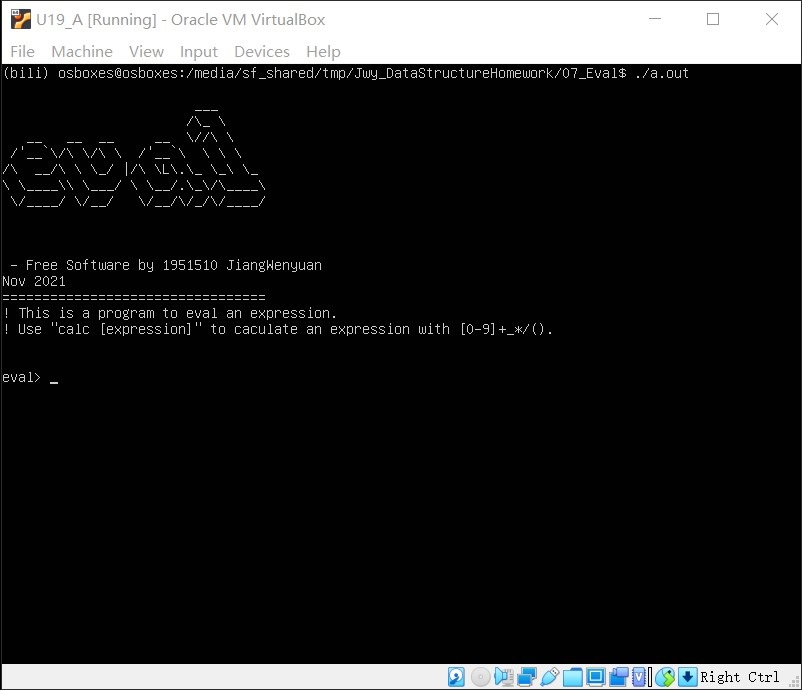
\includegraphics[width=0.7\linewidth]{image/e01.jpg}
    \caption{The user interface of the program}
\end{figure}

Usage of commands can be found on the main screen, and the \lstinline{help} command can give you information about theses commands.  All available commands is listed below.

\begin{enumerate}
    \item \lstinline{help} : Show help for a certain command.
    \item \lstinline{exit} : Exit the program.
    \item \lstinline{calc [expression]} : Process and calculate the given expression.
\end{enumerate}

\subsection{Calculate an expression}

Type \lstinline{calc 233+5*(1+(2+3)+6*2+(1))-5/6} to calculate a given expression.

\begin{figure}[H]
    \centering
    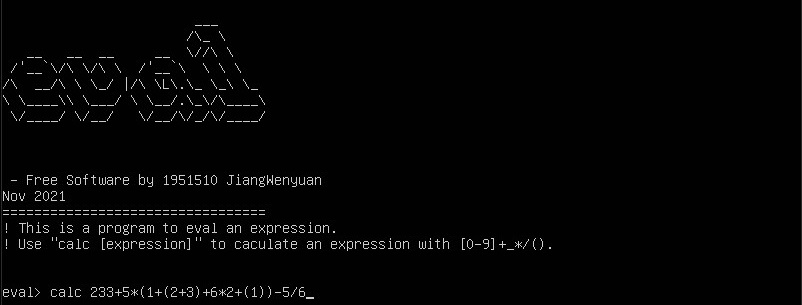
\includegraphics[width=0.7\linewidth]{image/e02.jpg}
    \caption{Evaluating an expression (1)}
\end{figure}
As can be seen, the expression tree, along with the answer and the postfix expression, infix expression is printed.
\begin{figure}[H]
    \centering
    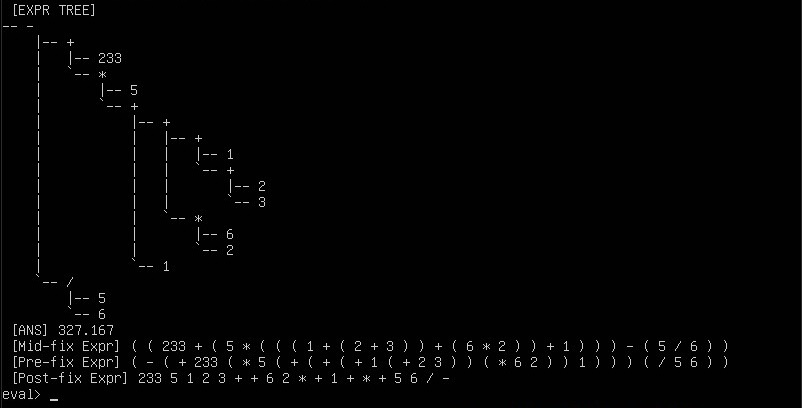
\includegraphics[width=0.7\linewidth]{image/e03.jpg}
    \caption{Evaluating an expression (2)}
\end{figure}


\section{The process of parsing an expression}

Previous researches on formal language and compilers have given out many powerful algorithms for parsing an expression. Two most famous algorithms, the LL(1)\uct{stearns1969property} and LR(1)\uct{wiki:Canonical_LR_parser} algorithms, are widely used in many compilers. However, implementation of these algorithms are relatively difficult by hand, since the parsers of common compilers are generated by utils like \lstinline{yacc} or \lstinline{bison}.

In this project, to make the implementation more straight forward, the generation of the Abstract Sytax Tree is a two stage process. The first stage deals with parentheses, and expressions are converted into a tree by the hierarchical relation of parentheses pairs. For example, the expression \lstinline{233+2*(3+4+9*(2+2)+(3+3))-5/6+1} is converted into a tree like this:
\begin{lstlisting}
-- EXP
    |-- 233
    |-- +
    |-- 2
    |-- *
    |-- EXP
    |   |-- 3
    |   |-- +
    |   |-- 4
    |   |-- +
    |   |-- 9
    |   |-- *
    |   |-- EXP
    |   |   |-- 2
    |   |   |-- +
    |   |   `-- 2
    |   |-- +
    |   `-- EXP
    |       |-- 3
    |       |-- +
    |       `-- 3
    |-- -
    |-- 5
    |-- /
    |-- 6
    |-- +
    `-- 1
\end{lstlisting}
with the sub expressions converted into a token named as \lstinline{EXP} for further processing. The second stage processes each layer of the previous tree, generating the final AST, which looks like this:
\begin{lstlisting}
-- +
    |-- -
    |   |-- +
    |   |   |-- 233
    |   |   `-- *
    |   |       |-- 2
    |   |       `-- +
    |   |           |-- +
    |   |           |   |-- +
    |   |           |   |   |-- 3
    |   |           |   |   `-- 4
    |   |           |   `-- *
    |   |           |       |-- 9
    |   |           |       `-- +
    |   |           |           |-- 2
    |   |           |           `-- 2
    |   |           `-- +
    |   |               |-- 3
    |   |               `-- 3
    |   `-- /
    |       |-- 5
    |       `-- 6
    `-- 1
\end{lstlisting}
Both steps of tree generation involves the manipulation of Stacks, which will be shown in the next section. After we have got the AST, different traversal algorithms of the gives out different types of expressions, and the AST can be evaluated recursively to give out the answer.

\section{Notes on the source code}

\paragraph{Pre-processing of user input} Since the user's input is a raw string, we first separate the string into basic components named tokens. Tokens have a type (NUM, ADD, SUB, MUL...), and for a number token, it has a value. The token is defined in the following code:
\begin{lstlisting}[language = C++]
struct raw_input
{
	node_type ch;
	double val;
......
};
vector<raw_input> ret;
\end{lstlisting}
The functions used to process the input is the \lstinline{split_input(string s)}, which resembles the lex analysis part of a compiler.

\paragraph{First stage of parsing}
The first parsing process is named as \lstinline{prase1(int l, int r)}, which is a recursive process to deal with parentheses. The most important part is shown below.
\begin{lstlisting}[language = C++]
p_node *prase1(int l, int r)
{
......
	stack<raw_input> s;
	int level = 0;
......
				res->child.push_back(prase1(s.top().pos + 1, i)); \\ Recursion HERE
				res->child.back()->parent = res;
			};
			s.pop();
			level--;
......
	};
	return res;
};
\end{lstlisting}
With the help of a stack, we can convert the token vector into a tree, but the tree need further processing to generate the final AST.

\paragraph{Second stage of parsing} is similar to the previous one, but it needs two stacks: the operater stack and the oprand stack, to deal with the expression with different priority levels. The logic of pushing and poping the stacks is more complex, which can be found in the source code.
\begin{lstlisting}[language = C++]
expr_node *prase2(p_node *r)
{
.....
	while (ptr < r->child.size())
	{
		switch (r->child[ptr]->op)
		{
		case NUM:
.....
		case RET:
.....
		case MUL:
.....
		case DIV:
.....
        exprs.push(prase2(s.top())); \\ Recursion HERE
.....
	return exprs.top();
};
\end{lstlisting}

\paragraph{Evaluation and printing} The evaluation and printing of the results are also recursive, since the AST is recursively defined. For example, to print the AST:
\begin{lstlisting}[language = C++]
int print_r_expr(expr_node *r, string sp)
{
	if (r == NULL)
	{
		return 0;
	};
......
		print_r_expr(r->op1, sp + "    ");
		print_r_expr(r->op2, sp + "    ");
	};
	return 0;
};
\end{lstlisting}
which is similar to the way we print the tree in the project \textit{Family Tree 家谱管理系统}.

The evaluation of the expression tree is also a recursive function. If the children of a node is not yet evaluated, then we recursively evaluate the children until all nodes have got their value. The code below shows the process:
\begin{lstlisting}[language = C++]
double eval(expr_node *r)
{
	if (r->is_evaled)
	{
		return r->val;
	}
	else if (r->op == NUM)
	{
......
	}
	else
	{
		double tmp;
		switch (r->op)
		{
		case ADD:
			tmp = (eval(r->op1) + eval(r->op2)); \\ Recursion HERE
......
		case SUB:
......
		case MUL:
......
		case DIV:
......
		default:
			break;
		};
		r->val = tmp;
		return r->val;
	};
};
\end{lstlisting}


Most of the code in \lstinline{main.cpp} is for processing the user's input, which is not so interesting.


\section{Discussion}

In this project, we built a simple parser for converting expression string to Abstract Sytax Tree for further evaluation and manipulation. Simple as it may seems to be, the hand written parser took several stacks, some recursive functions and a lot of if-s to implement. For a more complex language than an arithmetic expression, building a parser by hand is much more difficult.

In practice, these parsers to analysis the language is generated by some util tools, which are called "Compiler Compilers". Their input is the grammar rules written in Backus–Naur form\uct{wiki:Backus–Naur_form}, and they output the code that is used to parse the language to generate the AST. One of the widely used "Compiler Compilers" is \lstinline{Bison}, which is used in the \lstinline{GNU} project for building more complex compilers.\uct{aaby2003compiler}

Note that a simple but useful data structure, Stack, is widely used in the praser. The operations of a Stack with a set of rules are the key role of process a string to form the AST, which decides how to pop or push a stack according to the top element of each stack and the following input. The set of rules is given by the theory of Pushdown Automation and Regular Language, which will be learnt beyong the course of data structure (to be more precise, in compiler related courses).


\newpage
\bibliography{references}
\end{document}
